% {\color{red} \textbf{Đoạn text này để nói về mục đích và các công việc của chương này phải làm chứ không phải bình luận luôn kết quả ở đây => Viết lại nhé (xem phần mục tiêu ở chương 1). Nhấn mạnh rõ 2 mục đích của 2 loại thí nghiệm}:


Trong chương này, các mô phỏng lần lượt được thực hiện và trình bày. Thử nghiệm thuật toán tạo đường đi bao phủ RCPP trong vài khu vực khác nhau. Sau đó đánh giá hiệu suất giải pháp được đề xuất thông qua mô phỏng với mô hình robot chất điểm trên nền tảng viết bằng ngôn ngữ lập trình Python . Cuối cùng, các mô phỏng chứng minh tính khả thi của thuật toán bao phủ và đội hình đa robot trước khi nhúng lên robot thực tế được thực hiện trên trình mô phỏng vật lí Webots. 

\section{Mô phỏng tạo đường đi bao phủ}
% {\color{red} Lưu ý phân biệt giữa mCPP và RCPP. mCPP là dùng nói chung cho lập kế hoạch đường đi bao phủ của hệ thống đa robot còn RCPP là một kỹ thuật cụ thể để thực hiện mCPP.}

% Trong phần này, hiệu quả của thuật toán lập đường đi bao phủ cho đội hình chữ V được khảo sát trong đó tham số bao phủ của đội hình được tính theo mô hình trong hình \ref{fig:FOVmodel} (FOV của camera). 
% Bên cạnh đó, Kết quả sẽ được so sánh với thuật toán lập đường đi bao phủ khá gồmc 
% {\color{red} \textbf{ là.....} SO VỚI CÁI GÌ THÌ NÓI RÕ Ở ĐÂY: NÊN DÙNG 2 THUẬT TOÁN NHƯ TRONG PAPER} `\textbf{`grid-base coverage path planning''=> CÁI NÀY DỊCH LÀ PHƯƠNG PHÁP LẬP ĐƯỜNG ĐI BAO PHỦ DỰA TRÊN CHIA LƯỚI}
Trong phần này, hiệu quả của thuật toán lập đường đi bao phủ cho đội hình chữ V được khảo sát trong đó tham số bao phủ của đội hình được tính theo mô hình trong hình \ref{fig:FOVmodel} (FOV của camera). Thí nghiệm với ba bản đồ với các hình dạng, kích thước khác nhau đối với thuật toán bao phủ RCPP sẽ được tiến hành. Khoảng cách giữa $d_x$ các đường zig zac phụ thuộc vào vùng bao phủ của đội hình được tính dựa trên vùng bao phủ của từng robot và tỷ lệ trung lặp (overlapping) của vùng bao phủ giữa các robot kề nhau. Trong phần khảo sát này, khoảng cách $d_{x}$ được đưa ra cụ thể là: $12.17m$

Với bản đồ đầu tiên đường đi bao phủ đa robot được lập trong khu vực cần được khảo sát hình tứ giác với 4 điểm mốc lần lượt là x,y): (67.59, -21.76), (-23.44, -66.12), (-37.89, 74.93), (23.75, 43.96). Kết quả sẽ được trình bày trong Hình \ref{fig:o1} 
% {\color{red} TRONG QUYỂN TỌA ĐỘ NÊN BIỂU DIỄN CHÍNH XÁC ĐẾN 2 SỐ SAU DẤU PHẨY}
% \begin{figure}[H]
% \centering
%     \begin{subfigure}[b]{0.51\textwidth}
%     \centering
%     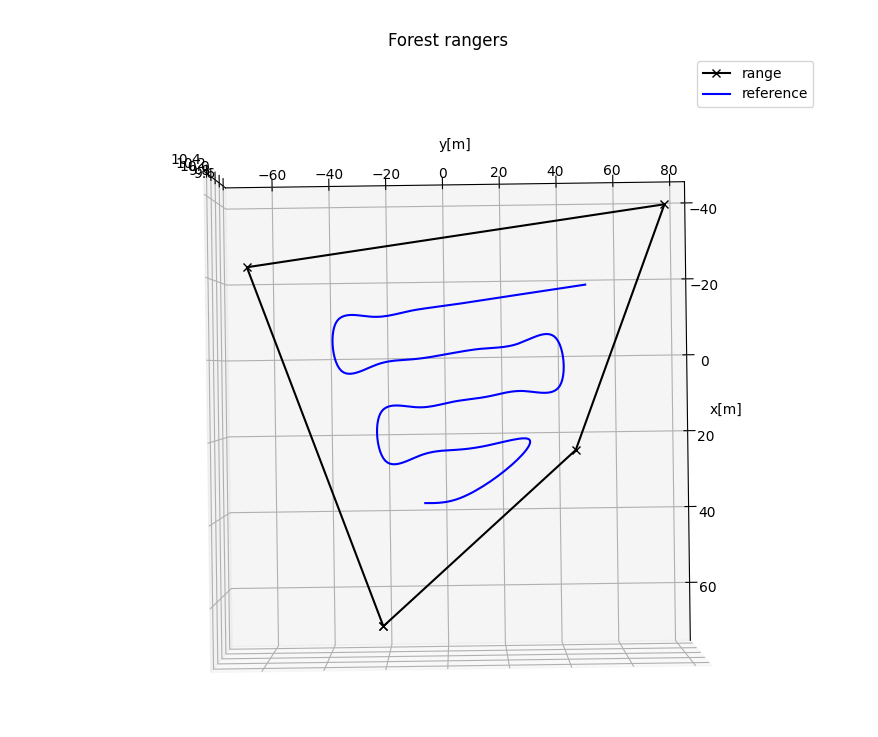
\includegraphics[width=\textwidth]{chapter5/image/anh1_grip.png}
%     \caption{Map 1 grip}
%     \label{fig:m1g}
%     \end{subfigure}
%     \hspace{0cm}
%     \begin{subfigure}[b]{0.45\textwidth}
%     \centering
%     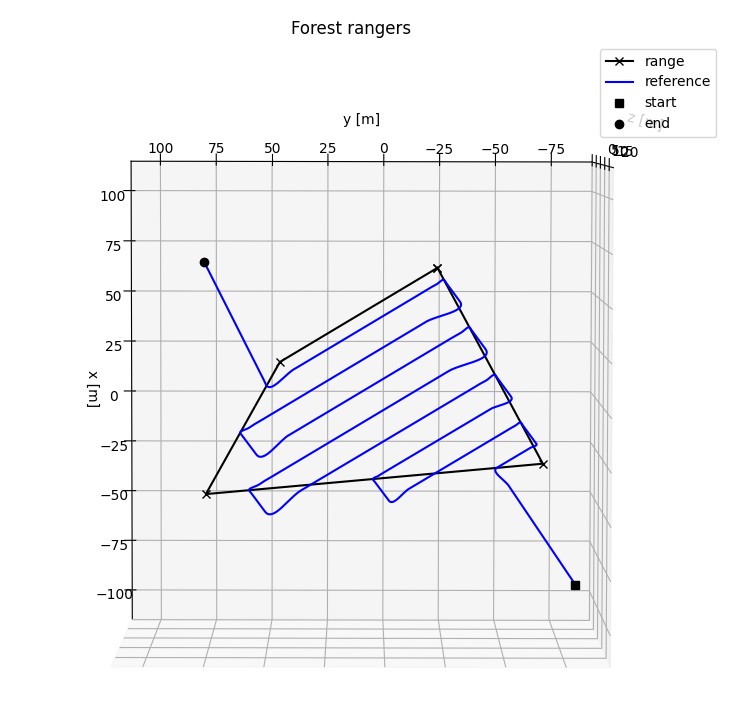
\includegraphics[width=\textwidth]{chapter5/image/anh1_op.png}
%     \caption{Map 1 op}
%     \label{fig:m1o}
%     \end{subfigure}
%     \captionsetup{justification=centering}
%     \caption{Map 1}
%     \label{fig:anh1}
% \end{figure}

\begin{figure}[h!]
    \centering
    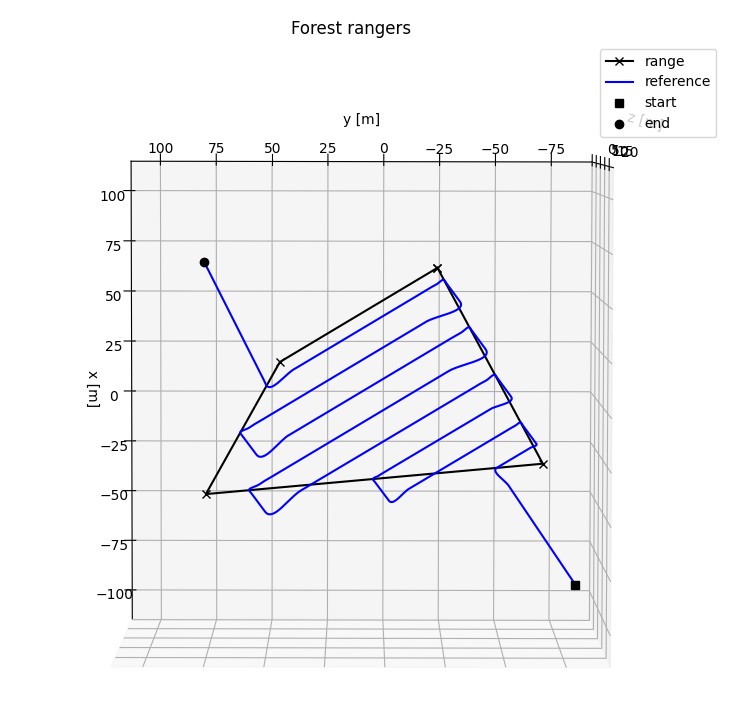
\includegraphics[width=0.68\textwidth]{chapter5/image/anh1_op.png}
    \caption{Bản đồ 1}
    \label{fig:o1}
\end{figure}

Với bản đồ thứ hai, khảo sát trên khu vực polygon hình ngũ giác được thực hiện với 5 điểm mốc (x,y) lần lượt là: (58.98, -40.46), (19.57, -78.53), (-62.67, 24.06), (-31.09, 61.08), (52.20, 26.41). Kết quả sẽ được trình bày trong Hình \ref{fig:o2}

% \begin{figure}[H]
% \centering
%     \begin{subfigure}[b]{0.45\textwidth}
%     \centering
%     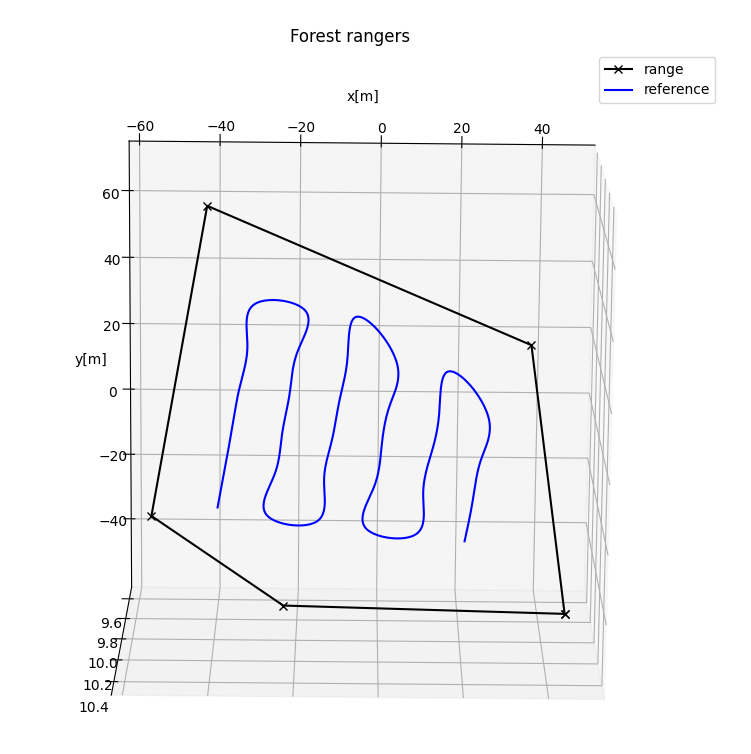
\includegraphics[width=\textwidth]{chapter5/image/anh2_grip.png}
%     \caption{Map 2 grip}
%     \label{fig:m1g}
%     \end{subfigure}
%     \hspace{0cm}
%     \begin{subfigure}[b]{0.50\textwidth}
%     \centering
%     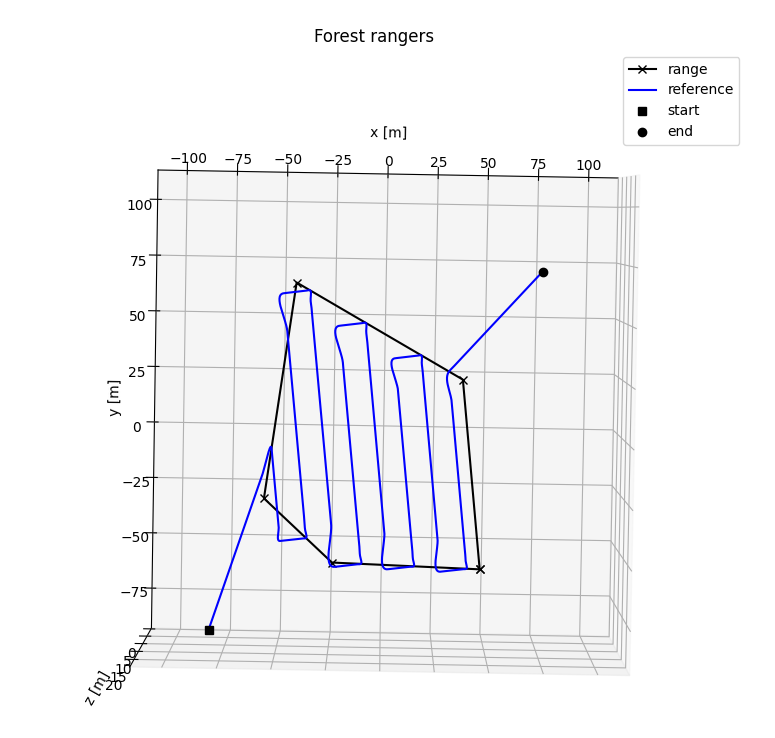
\includegraphics[width=\textwidth]{chapter5/image/anh2_op.png}
%     \caption{Map 2 op}
%     \label{fig:m1o}
%     \end{subfigure}
%     \captionsetup{justification=centering}
%     \caption{Map 2}
%     \label{fig:anh2}
% \end{figure}

\begin{figure}[h!]
    \centering
    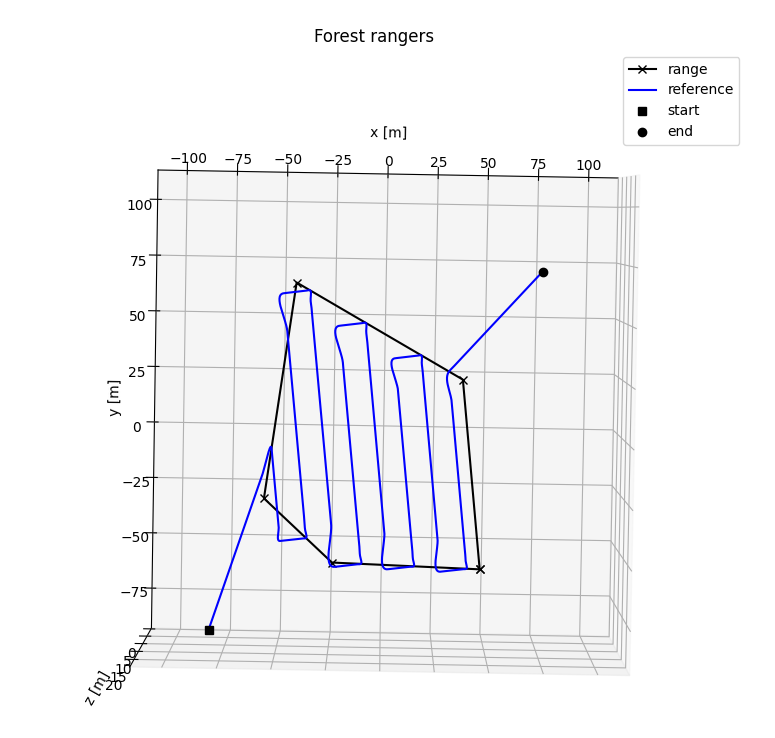
\includegraphics[width=0.68\textwidth]{chapter5/image/anh2_op.png}
    \caption{Bản đồ 2}
    \label{fig:o2}
\end{figure}


Cuối cùng với bản đồ thứ ba, khảo sát trên khu vực polygon hình lục giác với 6 điểm mốc (x,y) lần lượt là: (2.02, -3.39), (6.11, -52.97), (-31.21, -31.66), (-37.78, 9.98), (2.21, 52.65) ,(51.72, 8.25). Kết quả sẽ được trình bày trong Hình \ref{fig:o3}
% \begin{figure}
% \centering
%     \begin{subfigure}[b]{0.51\textwidth}
%     \centering
%     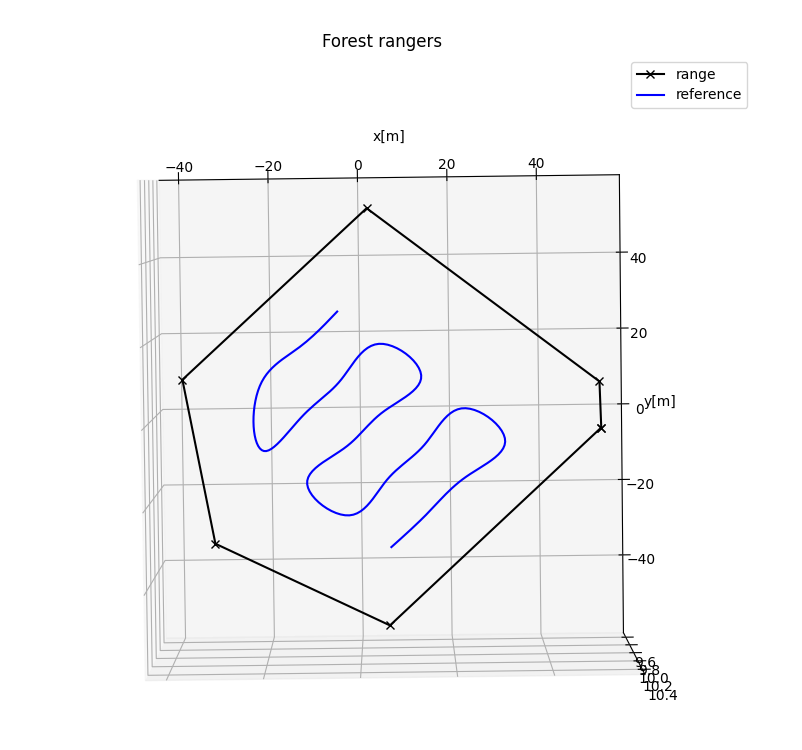
\includegraphics[width=\textwidth]{chapter5/image/anh3_grip.png}
%     \caption{Map 3 grip}
%     \label{fig:m1g}
%     \end{subfigure}
%     \hspace{0cm}
%     \begin{subfigure}[b]{0.46\textwidth}
%     \centering
%     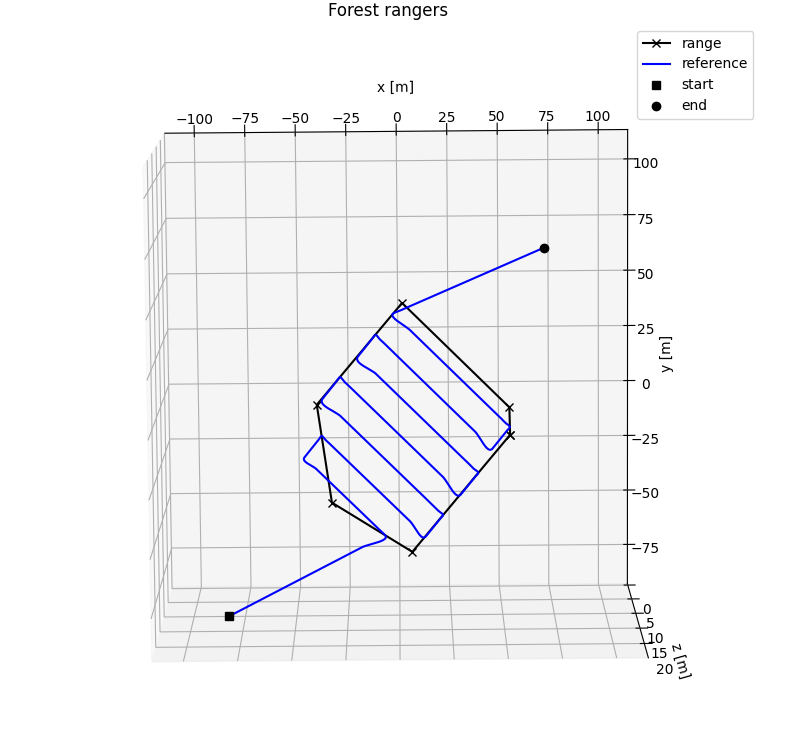
\includegraphics[width=\textwidth]{chapter5/image/anh3_op.png}
%     \caption{Map 3 op}
%     \label{fig:m1o}
%     \end{subfigure}
%     \captionsetup{justification=centering}
%     \caption{Map 3}
%     \label{fig:anh3}
% \end{figure}

\begin{figure}[h!]
    \centering
    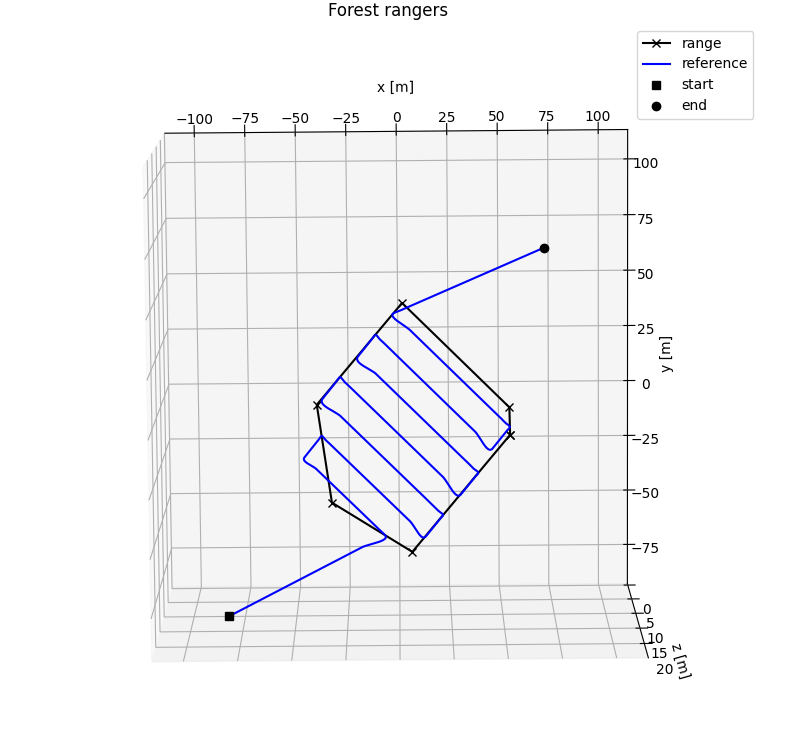
\includegraphics[width=0.68\textwidth]{chapter5/image/anh3_op.png}
    \caption{Bản đồ 3}
    \label{fig:o3}
\end{figure}

Tiến hành thực hiện với 3 khu vực khác nhau, thuật toán RCPP đều cho ra kết quả. Đường đi trong các hình đều xuất phát từ điểm bắt đầu và dừng lại ở điểm kết thúc, hoàn thiện được chu trình di chuyển của bầy robot quét qua toàn bộ khu vực. Nhờ đó mà có thể tính toán được không chỉ về mặt độ lớn quãng đường đi chính xác của robot là bao nhiêu mà còn tính toán được thời gian khảo sát phù hợp một cách tương đối chính xác.
% Ảnh bên trái là ảnh của quãng đường đi bao phủ của thuật toán GCPP và ảnh bên phải là hình ảnh kết quả của đường đi bao phủ mCPP. Do thuật toán GCPP đẩy vùng khảo sát từ tất cả các cạnh vào 1 khoảng bằng với dx, sau đó mới bắt đầu tiến hành chia lưới và khảo sát đường đi bao phủ tối ưu, nên kết quả thu được là một quỹ đạo chưa thực sự bao phủ hết được toàn bộ khu vực như thuật toán mCPP mà chỉ bao phủ được vùng trung tâm của khu vực. Ngoài ra thuật toán GCPP chưa tính đến điểm xuất phát và điểm kết thúc của các robot khảo sát nên quãng đường di chuyển chưa thực sự được tối ưu. Còn thuật toán mCPP quan tâm đến điểm bắt đầu và kết thúc, hoàn thiện được chu trình di chuyển của robot quét qua toàn bộ khu vực. Từ đó có thể tính toán được không chỉ về mặt độ lớn quãng đường đi chính xác của robot là bao nhiêu mà còn tính toán được thời gian khảo sát phù hợp một cách tương đối chính xác.

% Như vậy, qua các kết quả thu được, có thể thấy rằng thuật toán mCPP đạt hiệu quả hơn trong việc giải quyết vấn đề tìm đường đi bao phủ tối ưu trong một khu vực xác đinh. Bên cạnh đó, việc quan tâm đến điểm bắt đầu cũng như điểm kết thúc góp phần hình dung chính xác đường đường đi, quỹ đạo của robot trong quá trình khảo sát. 

% {\color{red} EM CÂN NHẮC KỸ NHÉ, THEO THẦY MỤC 3.1 NÀY CÓ THỂ KO CẦN VÌ HIỆU QUẢ CỦA THUẬT TOÁN LẬP KẾ HOẠCH PHẢI ĐƯỢC CHỨNG MINH THÔNG QUA KẾT QUẢ THỰC HIỆN CỤ THỂ BỞI ĐỘI HÌNH ROBOT. CÒN NẾU VẪN ĐỂ THÌ CẦN TÍNH TỶ LỆ BAO PHỦ CỤ THỂ CỦA TỪNG GIẢI PHÁP ĐỂ SO SÁNH. TÍNH TỈ LỆ BAO PHỦ TRONG CÁC TRƯỜNG HỢP NÀY HIỂU LÀ ĐỘI HINH ROBOT DI CHUYỂN LÝ TƯỞNG THEO ĐÚNG ĐƯỜNG THIẾT KẾ}